\documentclass[12pt]{article}
\newcommand\tab[1][1cm]{\hspace*{#1}}
\usepackage[utf8]{inputenc}
\usepackage{listings}
\usepackage{hyperref}
\usepackage{multirow}
\usepackage{color}
\usepackage{graphicx}
\pagenumbering{gobble}


\newcommand{\doubleSignature}[2]{
	\begin{center}
		
	\end{center}
	\vspace{2cm}
	
	\noindent
	\begin{tabular}{lcl}
		\rule{7cm}{1pt} & \hspace{2cm} & \rule{3cm}{1pt} \\
		#1 & & #2
	\end{tabular}
	\vspace{1cm}
}

\definecolor{codegreen}{rgb}{0,0.6,0}
\definecolor{codegray}{rgb}{0.5,0.5,0.5}
\definecolor{codepurple}{rgb}{0.58,0,0.82}
\definecolor{backcolour}{rgb}{0.95,0.95,0.92}

\hypersetup{
	colorlinks,
	citecolor=black,
	filecolor=black,
	linkcolor=black,
	urlcolor=black
}

\lstdefinestyle{mystyle}{
	backgroundcolor=\color{backcolour},   
	commentstyle=\color{codegreen},
	keywordstyle=\color{magenta},
	numberstyle=\tiny\color{codegray},
	stringstyle=\color{codepurple},
	basicstyle=\footnotesize,
	breakatwhitespace=false,         
	breaklines=true,                 
	captionpos=b,                    
	keepspaces=true,                 
	numbers=left,                    
	numbersep=5pt,                  
	showspaces=false,                
	showstringspaces=false,
	showtabs=false,                  
	tabsize=2
}

\lstset{style=mystyle}

\begin{document}
\begin{titlepage}
	

\author{Josef Bostik\\
	Eric Pereira\\
	Ryan Wojtlya\\}
\date{January 14\textsuperscript{th}, 2019}
\title{Project Plan}
\maketitle
\end{titlepage}
\tableofcontents
\newpage
\pagenumbering{arabic}

\section{Project Title}
\tab Upgrade and Update of Computer Systems within Dr. Hohlmann's High Energy Physics (HEP) Research Groups

\section{Names and Email Addresses of Team Members}
\tab
\begin{tabular}{| c | c |}
	\hline
	Joseph Bostik & \href{mailto: jbostik2015@my.fit.edu}{jbostik2015@my.fit.edu} \\
	\hline
	Eric Pereira & \href{mailto: epereira2015@my.fit.edu}{epereira2015@my.fit.edu} \\
	\hline
	Ryan Wojtyla & \href{mailto: rwojtyla2015@my.fit.edu}{rwojtyla2015@my.fit.edu} \\
	\hline
\end{tabular}

\section{Faculty Sponsor}
\tab Dr. Eraldo Ribeiro, \href{mailto: eribeiro@fit.edu}{eribeiro@fit.edu}

\section{Client}
\tab Dr. Marcus Hohlmann, \href{mailto: mhohlmann@fit.edu}{mhohlmann@fit.edu}

\section{Meeting(s) with the client for developing this plan}
\tab Weekly Monday meetings

\section{Goal and Motivation}
\tab The computer systems of the group have been in disarray for
some time, and these issues have been hindering the progress of
the group. The goal of the project is to repair and improve the
group’s resources to reduce the number of unnecessary obstacles
the group must overcome in order to conduct their research.
<<<<<<< HEAD
\section{Approach}
\subsection{Compute Cluster}
\subsection{Computer Systems}
\subsection{Muon Tomography Station (MTS)}

\section{Novel Features/Functionalities}
\subsection{Compute Cluster}
\subsection{Computer Systems}
\tab The computer systems in the HEP lab store important data locally on their systems that are crucial to their 
\subsection{MTS}
\subsubsection{Development MTS}
\subsubsection{Current MTS}
=======

\section{Approach}
	\subsection{Compute Cluster}
\tab The job of a computing cluster is to process both local jobs
submitted by researchers at FIT and jobs submitted via the Open
Science Grid, a platform through which researchers from around
the world may submit jobs to be processed. After installing
ROCKS, a distribution of CentOS specifically designed to easily
integrate all the components of a cluster, the next
step is to attach all the different components
of the compute cluster (SE, NAS's, etc.). Once the cluster is built,
HTCondor must be installed and configured to run jobs, then the
cluster must be reintegrated into the Open Science Grid to allow
for global job submissions. Scripts will also be written that ease
the process of locally submitting jobs.
	\subsection{Computer Systems}
		\tab The GEM team makes use of several different computers to
		both control hardware and take data. Most computers have been serviced
		and are currently in good use. However, some of the machines are
		still considered to be unreliable as they are not able to backup
		crucial data stored locally on the computers. The challenge currently
		is to find effective ways to create better storage methods, ideally
		using methods like RAID or integrating the computers with the compute
		cluster creating a GEM ecosystem.
	\subsection{Muon Tomography Station (MTS)}
		\subsubsection{Current MTS}
\tab The computer managing the (MTS) is encumbered by heavily outdated software that dramatically hinders its basic operation. Additionally, the workflow for taking data from the MTS is
comprised of several loosely connected programs and scripts that
are difficult to manage and do not provide diagnostic information
about the data taking process. The management computer’s software must be brought up to date, and the data taking workflow must be rewritten to allow for troubleshooting capabilities.
		\subsubsection{Development MTS}
\tab The computer managing the (MTS) is encumbered by heavily outdated software that dramatically hinders its basic operation. Additionally, the workflow for taking data from the MTS is
comprised of several loosely connected programs and scripts that
are difficult to manage and do not provide diagnostic information
about the data taking process. The management computer’s software must be brought up to date, and the data taking workflow must be rewritten to allow for troubleshooting capabilities.


\section{Novel Features/Functionalities}
\subsection{Compute Cluster}
\tab The streamlined submission of jobs to a functioning computing
cluster in order to ease data processing.
\subsection{Computer Systems}
\tab The introduction of updated and better supported computer systems to the GEM team’s
collection of machines.
\subsection{MTS}
The creation of a new data taking workflow for the MTS that
includes troubleshooting capabilities so that data taking issues can
more quickly be diagnosed.

>>>>>>> 5ee1e0b4f345f7e0bfaed17b7ebdccdfd222fc61


\section{Technical Challenges}
\subsection{Compute Cluster}
<<<<<<< HEAD
\subsection{Computer Systems}
\tab The computer systems in the lab hold major data that is only stored locally on very specific computers. The issue here is that a lot of these computers do not have a backup of their data somewhere else which means that if there is a major hard drive failure lots of data will be lost. The ideal solution to this is to run all machines in RAID 1 with two hard drives in each machine, which will striped all data on one hard drive to another creating a backup. 
\subsection{MTS}
\subsubsection{Development MTS}
\tab The development MTS currently has a major issue with the installation of AMORE
\subsubsection{Current MTS}
\tab The current MTS currently has a major issue where one of the FEC's is unusable due to bad firmware. Having one bad FEC renders the entire MTS useless due to how the software on the MTS computer currently works. \\
\tab Another technical challenge with the current MTS is hardware wiring. The wiring of the MTS is disasterous, and makes it very difficult to unplug and and plug in other ports without losing track of cables, or putting cables in the wrong spot. This is because many cables are not labelled, and some cables are as long as 30 feet even when they are only connecting things roughly three to six feet away. 
=======
\tab The computer cluster has recently had an operating, ROCKS, installed on the system. Although ROCKS is installed on the CE (Computing Element) of the cluster it has yet to also integrate the Storage Element (SE) and the Network Assisted Storage (NAS). After this is getting HTCondor installed, and connecting to the Open Science Grid (OSG) so that it can take jobs and complete them. 
\subsection{Computer Systems}
\tab The computer systems in the lab hold major data that is only stored locally on very specific computers. The issue here is that a lot of these computers do not have a backup of their data somewhere else which means that if there is a major hard drive failure lots of data will be lost. The ideal solution to this is to run all machines in RAID 1 with two hard drives in each machine, which will striped all data on one hard drive to another creating a backup. 
\subsection{MTS}
\subsubsection{Current MTS}
\tab The current MTS currently has a major issue where one of the FEC's is unusable due to bad firmware. Having one bad FEC renders the entire MTS useless due to how the software on the MTS computer currently works. \\
\tab Another technical challenge with the current MTS is hardware wiring. The wiring of the MTS is disasterous, and makes it very difficult to unplug and and plug in other ports without losing track of cables, or putting cables in the wrong spot. This is because many cables are not labelled, and some cables are as long as 30 feet even when they are only connecting things roughly three to six feet away.
\subsubsection{Development MTS}
\tab The development MTS has been having a few software issues, specifically with running AMORE with the DATE software. This is a challenge as there is not much documentation as to the process of installing these softwares with the new supported operating system of CERN: CentOS 7.
 
>>>>>>> 5ee1e0b4f345f7e0bfaed17b7ebdccdfd222fc61
\section{Design}
\subsection{Compute Cluster}
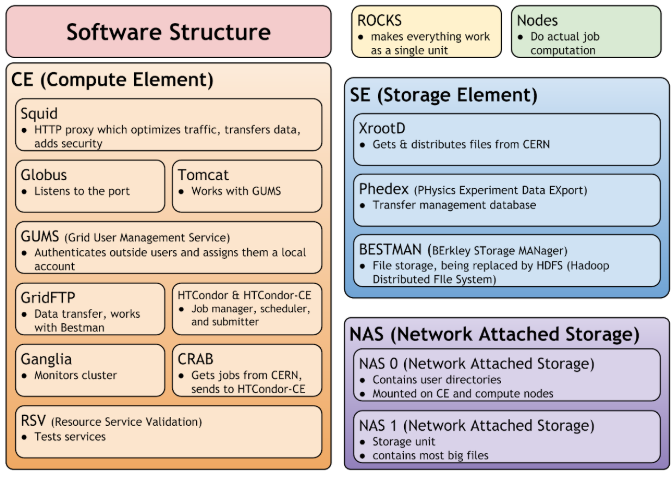
\includegraphics{Cluster_Design_Image.png}
\subsection{MTS}
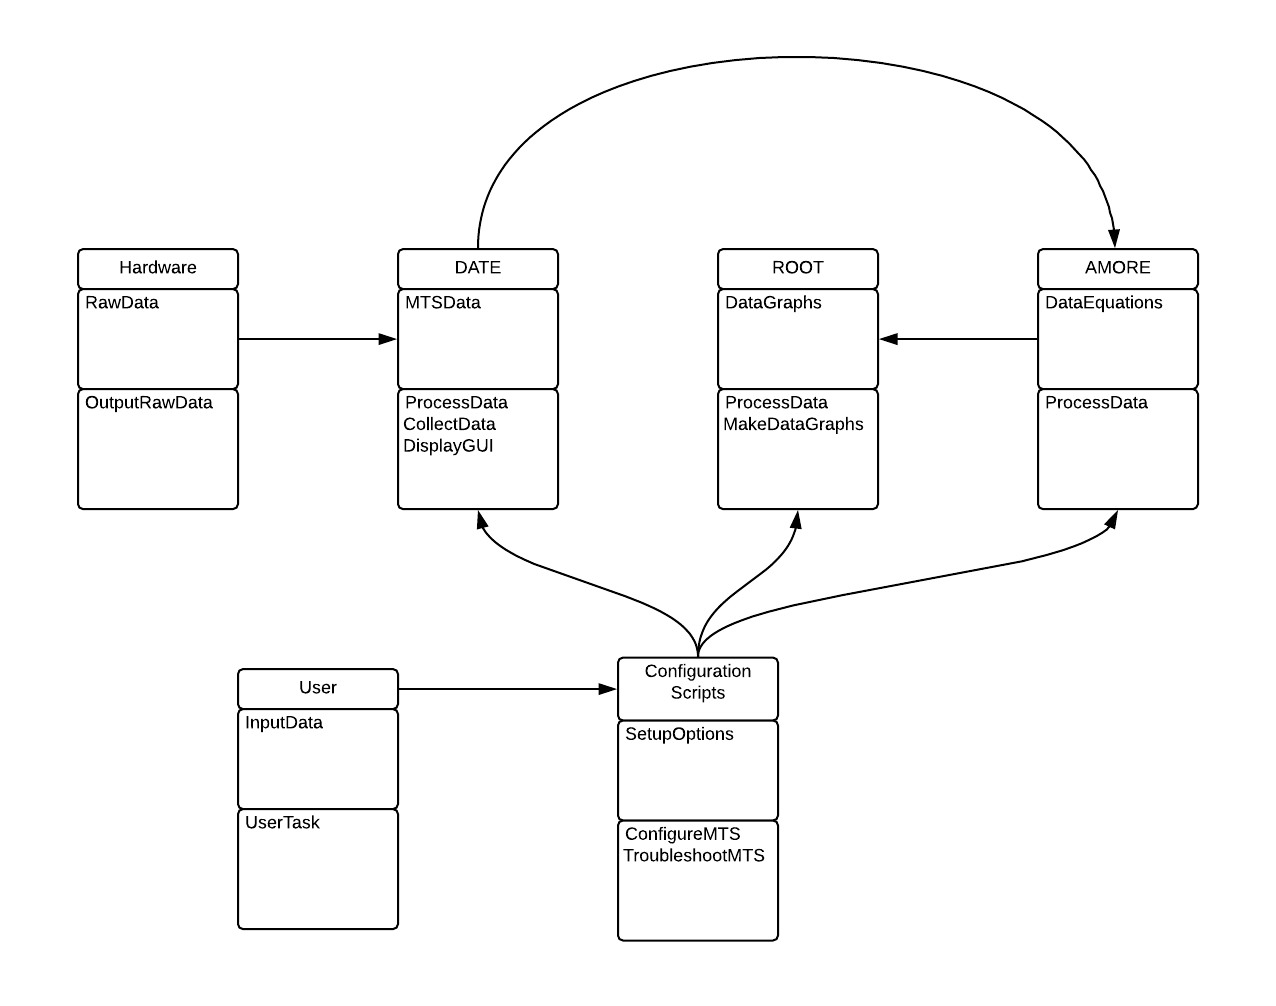
\includegraphics[scale=.75]{image3.png}
\section{Progress Summary}

\section{Table of Major Goals}
\begin{tabular}{|c|c|c|}
	\hline
	Model/Feature & Completion \% & To Do \\
	\hline
	Install ROCKS on Cluster & 60\% & Need to integrate all parts \\
	\hline
	Replace Current MTS & 50\% & Install AMORE on dev MTS \\
	\hline
	MTS Automated Script & 50\% & use DATE \& AMORE in mock script \\
	\hline
	Reallocate Hardware & 100\% & N/A \\
	\hline
	GEM Computer backups & 50\% & Get cluster NAS online \\
	\hline
	
\end{tabular}
\subsection{Compute Cluster}
\tab Originally the compute cluster was in complete Disarray, and did not work at all. The plan was to rebuild it from scratch, starting by putting a new operating system on the system. This ended up being problematic as there was a lot of trouble being able to simply access the CE initially. Eventually we were able to read and access the individual parts of the cluster, and install ROCKS operating system on the computer cluster. 
\subsection{Computer Systems}
\tab The computer systems of the lab are in better shape than they previously were, The reallocation of resources has allowed for hardware, such as memory or video cards, to be placed in PC's for their specific use. For example: The development MTS does not need much graphical power as it runs math equations and makes small 2 dimensional graphs, so integrated graphics are fine for it, but another PC like the Beauty PC requires it for 3D modeling. \\
\tab With the computer systems there is also a smalls script that was created for software that mimics on a small scale what the MTS does on a large scale. This script has an Alias in the bash terminal to run it, and runs all the commands and uses given inputs in order to run the software to create 2 dimensional live graphs of what it can see in a scaled down MTS system. This software could be useful in creating the script necessary the MTS.
\subsection{MTS}
\subsubsection{Current MTS}
\tab The current MTS was fixed shorty after taking upon the project. Going into and rewriting a few config files allowed for the MTS to be used again and collect data. This progress allowed the group to take data, which led to the creation of the Development MTS, a computer in which the latest versions of all supported hardware will be installed and to manufacture the script in order to automate tasks. \\
\tab Although all seemed well, it appears that one of the FEC/ADC cards (a card which is allows for readout from the MTS) ended up failing, and the DAQ software needs to have 6 supported FEC's in order to work. With this failure we only had 5 FEC's. There was conveniently a spare FEC, but it seems to have outdated firmware that is not supported by the DAQ software, so that needs to be updated. 
\subsubsection{Development MTS}
\tab The development MTS is a project taken up to be used and replace the current MTS PC. The reason for this is that the Current MTS is horribly outdated, and the way that the current MTS is configured it is impossible to update or upgrade the software and OS without completely starting from scratch. Due to the current MTS still working and being able to take data, it was decided with our advisor that one of the spare PC's in the lab could be used as a development PC for the MTS. \\
\tab The development MTS has installed the version of CentOS supported by CERN, along with all the necessary software to get started. DATE/DAQ data taking software has been installed and works, and AMORE was also installed and works, but the two do not seem to sync together as they have to have specific versions to communicate with each other.


\section{Milestone 4 (Feb 11)}
<<<<<<< HEAD

\section{Milestone 5 (Mar 18)}

\section{Milestone 6 (April 15)}
=======
\begin{itemize}
	\item Integrate all parts of the cluster together
	\item Rewire the current MTS and clean up the cables 
	\item fix the current version of AMORE on the development MTS
\end{itemize}

\section{Milestone 5 (Mar 18)}
\begin{itemize}
	\item Install HTCondor and connect the cluster to OSG
	\item Create Automated Script for MTS on the development machine
	\item Find Effective ways to make backups for GEM computers
\end{itemize}

\section{Milestone 6 (April 15)}
\begin{itemize}
	\item Replace Current MTS with Development MTS
	\item Create the Showcase Poster
	\item Create a Showcase video showing our progress
	\item Finalize progress with Advisor
\end{itemize}
>>>>>>> 5ee1e0b4f345f7e0bfaed17b7ebdccdfd222fc61

\section{Task Matrix for Milestone 4}
\begin{tabular}{| c | c | c | c |}
	\hline 
	Task & Josef Bostik & Eric Pereira & Ryan Wojtyla \\
	\hline 
	Rewire Current MTS & 30\% & 40\% & 30\% \\
	\hline 
	Fix AMORE installation & 70\% & 0\% & 30\% \\
	\hline
	Attach SE \& NAS to Cluster & 10\% & 20\% & 70\% \\
	\hline
	Find backup solution & 0\% & 80\% & 20\% \\
	\hline
	
\end{tabular}


<<<<<<< HEAD
=======
\section{Description of each planned task for Milestone 4}
\subsection{Compute Cluster}
\tab Integrate each part of compute cluster with ROCKS so that they can all communicate with each other.
\subsection{Computer Systems}
\tab Finding an effective way to backup for each of the computers so that in the case of catastrophic hard drive failure data will be recoverable. 
\subsection{MTS}
\subsubsection{Current MTS}
\tab Rewire the current MTS so that it is clean, organized in the case that something needs to be unplugged, and provides a cleaner Aesthetic in the lab. 
\subsubsection{Development MTS}
\tab The version of AMORE on the computer currently is not supported and working with the DAQ/DATE and is having some issues working. In order to use the software we have to find out what the issue is, and fix AMORE so that it will work with DATE/DAQ to read in data. 

>>>>>>> 5ee1e0b4f345f7e0bfaed17b7ebdccdfd222fc61
\section{Approval from Faculty Sponsor}
\paragraph{\tab "I have discussed with the team and approve this project plan. I will evaluate the progress and assign a grade fo reach of the three milestones"}
\doubleSignature{Signature}{Date}

\end{document}
